
%\documentclass[10pt,a5paper,fleqn]{article}
%\usepackage[utf8]{inputenc}
%\usepackage{amssymb, amsmath, multicol}
%\usepackage[russian]{babel}
%\usepackage{graphicx}
%\usepackage[shortcuts,cyremdash]{extdash}
%\usepackage{wrapfig}
%\usepackage{floatflt}
%\usepackage{lipsum}
%\usepackage{concmath}
%\usepackage{euler}

\documentclass[a4paper,12pt]{article} % тип документа


% Русский язык
\usepackage[warn]{mathtext}
\usepackage[T2A]{fontenc} % кодировка
\usepackage[utf8]{inputenc} % кодировка исходного текста
\usepackage[russian,english]{babel} % локализация и переносы
\usepackage{graphicx}
\DeclareGraphicsExtensions{.pdf,.png,.jpg}


\graphicspath{ {images/} }
\setlength{\parskip}{0.5cm}

% Математика
\usepackage{amsmath,amsfonts,amssymb,amsthm,mathtools}


\usepackage{wasysym}

%Заговолок
\author{}

\title{}

\date{}

\begin{document}

%\maketitle
%\thispagestyle{empty}

%\newpage
\setcounter{page}{1}



\begin{center}
  \LARGE{Лабораторная работа 2.5.1}\\[0.2cm]
  \LARGE{Измерение коэффициента поверхностного натяжения жидкости.}\\[0.2cm]
  \large{10 Февраля 2021 г.}\\[0.2cm]
  \large{Старченко Иван Александрович}\\[0.2cm]
\end{center}

\textbf{Цель работы:} \\
1) измерение температурной зависимости  коэффициента поверхностного натяжения дистиллированной воды с использованием известного коэффициента поверхностного натяжения спирта;  \\
2) определение полной поверхностной энергии  и теплоты, необходимой для изотермического образования единицы  поверхности жидкости  при различной температуре. 


\begin{center}
	\large{\textbf{Теоретические сведения}}
\end{center}

Наличие поверхностного слоя приводит к различию давлений по разные стороны от искривленной границы раздела двух сред.  Для сферического пузырька с воздухом  внутри жидкости избыточное давление даётся формулой Лапласа:

\begin{equation}
	\Delta P = P_{inside} - P_{outside} = \frac{2\sigma}{r},
\end{equation}

где $\sigma$ – коэффициент поверхностного натяжения, $P_{inside}$ и $P_{outside}$ – давление внутри пузырька и снаружи, r – радиус кривизны поверхности раздела двух фаз. Эта формула лежит в основе предлагаемого метода определения коэффициента поверхностного натяжения жидкости. Измеряется давление $\Delta P$, необходимое для выталкивания в жидкость пузырька воздуха.

\begin{center}
	\large{\textbf{Экспериментальная установка}}
\end{center}

Исследуемая жидкость (дистиллированная вода) наливается в сосуд (колбу) В. Тестовая жидкость  (этиловый спирт) наливается  в сосуд Е.  При измерениях  колбы герметично закрываются  пробками.   Через одну из двух пробок  проходит полая металлическая игла С. Этой пробкой закрывается сосуд, в котором  проводятся измерения. Верхний конец иглы открыт в атмосферу, а нижний погружен в жидкость. Другой сосуд герметично закрывается второй пробкой. При создании достаточного  разряжения воздуха в колбе с иглой пузырьки воздуха начинают пробулькивать через жидкость. Поверхностное натяжение можно определить по величине разряжения P1, необходимого для прохождения пузырьков (при известном радиусе иглы).


Разряжение в системе создается с помощью аспиратора А. Кран К2 разделяет две полости аспиратора. Верхняя полость при закрытом кране К2  заполняется водой. Затем кран К2 открывают и заполняют водой  нижнюю полость  аспиратора.  Разряжение воздуха создается в нижней полости  при открывании крана К1, когда  вода вытекает из неё по каплям. В колбах В и С, соединённых трубками с нижней полостью аспиратора,  создается такое же пониженное давление. Разность давлений в полостях с разряженным воздухом и атмосферой измеряется спиртовым микроманометром (устройство микроманометра описано в Приложении). 
Для стабилизации температуры исследуемой жидкости через рубашку D колбы В непрерывно прогоняется вода из термостата.

\includegraphics[width=1\textwidth]{Scheme.jpg}

Обычно кончик иглы лишь касается поверхности жидкости, чтобы исключить влияние гидростатического давления столба жидкости. Однако при измерении температурной зависимости коэффициента поверхностного натяжения возникает ряд сложностей. Во-первых, большая теплопроводность металлической трубки приводит к тому, что температура на конце трубки заметно ниже, чем в глубине жидкости. Во-вторых, тепловое расширение поднимает уровень жидкости при увеличении температуры. 

Обе погрешности можно устранить, погрузив кончик трубки до самого дна. Полное давление, измеренное при этом микроманометром, $P = \Delta P + \rho gh$. Заметим, что $\rho gh$ от температуры практически не зависит, так как подъём уровня жидкости компенсируется уменьшением её плотности (произведение $\rho h$ определяется массой всей жидкости и поэтому постоянно). Величину  $\rho gh$ следует измерить двумя способами. Во-первых, замерить величину $P1 = \Delta P'$, когда кончик трубки только касается поверхности жидкости. Затем при этой же температуре опустить иглу до дна и замерить $P2 = \rho gh + \Delta P"$ ($\Delta P' ,\: \Delta P"$ – давление Лапласа). Из-за  несжимаемости  жидкости можно положить $\Delta P' = \Delta P"$ и тогда $\rho gh = P2 -P1$. Во-вторых, при измерениях $Р1$ и $Р2$ замерить линейкой  глубину погружения иглы $h$. Это можно сделать, замеряя расстояние между верхним концом иглы и любой неподвижной частью прибора при положении иглы на поверхности и в глубине колбы.

\begin{center}
	\large{\textbf{Измерения}}
\end{center}

1) Убедившись в герметичности системы, начал измерения. Открыл кран К1. Подобрал частоту падения капель не чаще, чем 1 капля в 5 секунд. 

2) Измерил высоту подъема спирта $\Delta h$  при  пробулькивании пузырьков воздуха на поверхности спирт. Снятые данные занёс в таблицу:

\begin{tabular}{ | c | c | c | c | c | c |c | c | c | c | c | }
\hline
	N              & 1  & 2  & 3  & 4  & 5  & 6  & 7  & 8  & 9  & 10 \\ \hline
	$\Delta h$, мм & 47 & 46 & 47 & 48 & 47 & 47 & 47 & 48 & 47 & 46 \\ \hline
\end{tabular}\\
\setlength{\parskip}{0.3cm}\\
Таблица 1: Измерение давления пузырьков на поверхности спирта

Посчитал среднее значение и оценил случайную и систематическую погрешность: 
\[<\Delta h>\ = \frac{47+46+47+48+47+47+47+48+47+46}{10} = 47.0\ \text{мм}\]
\[\delta_{<\Delta h> \text{случ}} = \sqrt{\frac{1}{n(n-1)}\sum_{i=1}^n(\Delta h_i - <\Delta h>)^2} = \sqrt{\frac{1}{10(10-1)}\sum_{i=1}^{10}(\Delta h_i - 47.0)^2} = 0.2\ \text{мм}\]

\[\delta_{<\Delta h> \text{сист}} = 1.0\ \text{мм}\]

Полная погрешность измерения:
\[\delta_{<\Delta h>} = \sqrt{\delta_{<\Delta h> \text{сист}}^2 + 
							  \delta_{<\Delta h> \text{случ}}^2} \approx 1.0\ \text{мм}\]
							  
Перейдем по формуле (1):$\displaystyle P = C\cdot \frac{\gamma_\text{сп. залит}}{\gamma_\text{сп. пр}}\cdot K\cdot h\cdot 9.81$( где $P$ -- давление в Па, $C$ -- поправочный множитель, $h$ -- отсчет по шкале, $K$ -- постоянная ушла наклона, $\gamma_\text{сп. залит}$ -- плотность спирта залитого в прибор, $\gamma_\text{сп. пр}$ -- плотность спирта указанного на приборе) от высоты к давлнию:

\[P = 1.0\cdot \frac{0.8066}{0.8095}\cdot 0.2\cdot 47.0\cdot 9.81\approx 91.88\ \text{Па}\]

\[\delta_P = 1.0\cdot \frac{0.8066}{0.8095}\cdot 0.2\cdot 1.0\cdot 9.81\approx 1.95\ \text{Па}\]

Тогда получаем:
\[P = (91.88 \pm 1.95)\ \text{Па}\]

Приняв за табличное значение коэффициента поверхностного наятжения спирта величину $\sigma = 0,0228\ \text{H/м}$, расчитаем диаметр иглы:
\[d = \frac{4\sigma}{P} = 0.99\ \text{мм}\]
\[\delta_d = d\cdot \frac{\sigma_p}{P} \approx 0.02\ \text{мм}\]
\[d = (0.99 \pm 0.02)\ \text{мм}\]

Диаметр трубки, измеренный с помощью микроскопа и линейки, равен $(0.97 \pm 0.01)\ \text{мм}$. В дальнейшем будем пользоваться им. Также стоит отметить, что косвенное измерение диаметра достаточно близко к прямому измерению, что говорит о применимости данного метода.

\setlength{\parskip}{0.5cm}

3) Промоем, высушим и перенесем иглу в колбу с дистиллированной водой. Теперь измерим максимальное давление $P_1$ при пробулькивании пузырьков, когда игла лишь касается поверхности воды, также измерим расстояние между верхним концом иглы и пробкой пробирки $h_1$.

\begin{tabular}{ | c | c | c | c | c | c |c | c | c | c | c | }
\hline
	N  & 1  & 2  & 3  & 4  & 5  & 6  & 7  & 8  & 9  & 10 \\ \hline
	$\Delta h_1$, мм & 119 & 119 & 119 & 120 & 119 & 119 & 119 & 118 & 119 & 119 \\ \hline
\end{tabular}\\
\setlength{\parskip}{0.3cm}\\
Таблица 2: Измерение давления пузырьков на поверхности воды

Аналогично пункту 2 найдем полную погрешность:
\[<\Delta h_1>\ = \frac{119+119+119+120+119+119+119+118+119+119}{10} = 119.0\ \text{мм}\]
\[\delta_{<\Delta h_1> \text{случ}} = \sqrt{\frac{1}{n(n-1)}\sum_{i=1}^n(\Delta h_i - <\Delta h_1>)^2} = \sqrt{\frac{1}{10(10-1)}\sum_{i=1}^{10}(\Delta h_i - 119.0)^2} = 0.2\ \text{мм}\]

\[\delta_{<\Delta h_1> \text{сист}} = 1.0\ \text{мм}\]

Полная погрешность измерения:
\[\delta_{<\Delta h_1>} = \sqrt{\delta_{<\Delta h_1> \text{сист}}^2 + 
							  \delta_{<\Delta h_1> \text{случ}}^2} \approx 1.0\ \text{мм}\]
							  
Перейдем по формуле (1): от высоты к давлнию:
\[P_1 = 1.0\cdot \frac{0.8066}{0.8095}\cdot 0.2\cdot 119.0\cdot 9.81\approx 232.64\ \text{Па}\]

\[\delta_{P_1} = 1.0\cdot \frac{0.8066}{0.8095}\cdot 0.2\cdot 1.0\cdot 9.81\approx 1.95\ \text{Па}\]

Тогда получаем:
\[P_1 = (232.64 \pm 1.95)\ \text{Па}\]

Расстояние между верхним концом иглы и пробкой пробирки $h_1$ равно $(5.5 \pm 0.1)\ \text{cм}$

4) Опустим теперь иглу практически до дна, расстояние между верхним концом иглы и пробкой пробирки $h_2$ равно $(6.8 \pm 0.1)\ \text{cм}$, тогда:
\[\Delta h_1 = h_2 - h_1 = (1.3 \pm 0.1)\ \text{см}\]

Аналогично предыдущим пунктам найдем давление пузырьков на дне воды:

\begin{tabular}{ | c | c | c | c | c | c |c | c | c | c | c | }
\hline
	N  & 1  & 2  & 3  & 4  & 5  & 6  & 7  & 8  & 9  & 10 \\ \hline
	$\Delta h_2$, мм & 181 & 181 & 181 & 181 & 181 & 181 & 181 & 181 & 181 & 181 \\ \hline
\end{tabular}\\
\setlength{\parskip}{0.3cm}\\
Таблица 3: Измерение давления пузырьков на дне пробирки
\[<\Delta h_2>\ = \frac{181+181+181+181+181+181+181+181+181+181}{10} = 181.0\ \text{мм}\]
\[\delta_{<\Delta h_2> \text{случ}} = \sqrt{\frac{1}{n(n-1)}\sum_{i=1}^n(\Delta h_i - <\Delta h_1>)^2} = \sqrt{\frac{1}{10(10-1)}\sum_{i=1}^{10}(\Delta h_i - 181.0)^2} = 0.0\ \text{мм}\]

\[\delta_{<\Delta h_2> \text{сист}} = 1.0\ \text{мм}\]

Полная погрешность измерения:
\[\delta_{<\Delta h_2>} = \sqrt{\delta_{<\Delta h_2> \text{сист}}^2 + 
							  \delta_{<\Delta h_2> \text{случ}}^2} \approx 1.0\ \text{мм}\]
							  
Перейдем по формуле (1): от высоты к давлнию:

\[P_2 = 1.0\cdot \frac{0.8066}{0.8095}\cdot 0.2\cdot 181.0\cdot 9.81\approx 353.85\ \text{Па}\]

\[\delta_{P_2} = 1.0\cdot \frac{0.8066}{0.8095}\cdot 0.2\cdot 1.0\cdot 9.81\approx 1.95\ \text{Па}\]

Тогда получаем:
\[P_2 = (353.85 \pm 1.95)\ \text{Па}\]

Найдем $\Delta h_2$ косвенным методом:
\[\Delta h_2 = \frac{P_2-P_1}{\rho g},\]

где $\rho = 998,2\ kg/m^3$ -- плотность дистиллированной воды, а $g = 9.81\
 \text{Н/м}$ -- ускорение свободного падения.
 
\[\Delta h_2 = 1.24 \text{см}\]
\[\delta_{\Delta h_2} = \Delta h\cdot \frac{\delta_P}{P_2 - P_1}\]

\[\delta_{\Delta h_2} = 1.2\cdot \frac{1.95}{121.20} = 0.02 см\]

Cравним значения $\Delta h_1$ и $\Delta h_2$. $\Delta h_1 = (1.3 \pm 0.1)\ \text{см}$, а $\Delta h_2 = (1.24 \pm 0.02)\ \text{см}$. Значение $\Delta h_2$ более точное, при надобности будем пользоваться им.

Снимим температурную зависимость $\sigma(T)$ дистиллированной воды. Для расчета используем формулу, при этом $d$ будет та, которую мы меряли с помощью микроскопа и линейки, а именно $d = (0.97 \pm 0.01) $ мм:
\[\sigma(T) = \frac{(P-\Delta P)\cdot d}{4}\]

\begin{tabular}{ | c | c | c | c | c | c | c | c |}
\hline
 $N$ & $T, C^{\circ}$ & $T, K$  & $\Delta h,$ мм & $P$, Па & $\Delta P$, Па & 
 $P - \Delta P$, Па  & $\sigma$ Дж/м$^2$   \\ \hline
1& 20.1 & 293.3 & 181 & 353.85 & 121.21 & 232.64 & 0.0564  \\ \hline
2& 30.2 & 303.4 & 180 & 351.89 & 121.21 & 230.68 & 0.0559  \\ \hline
3& 35.2 & 308.4 & 178 & 347.98 & 121.21 & 226.77 & 0.0550  \\ \hline
4& 40.2 & 313.4 & 177 & 346.02 & 121.21 & 224.81 & 0.0545  \\ \hline
5& 45.2 & 318.4 & 176 & 344.07 & 121.21 & 223.86 & 0.0542  \\ \hline
6& 50.2 & 323.4 & 175 & 342.11 & 121.21 & 220.90 & 0.0536  \\ \hline
7& 55.2 & 328.4 & 174 & 340.16 & 121.21 & 218.95 & 0.0531  \\ \hline
\end{tabular}\\
\setlength{\parskip}{0.3cm}\\
Таблица 4: Температурная зависимость коэффициента поверхностного натяжения

Расчитаем погрешность:
\[\delta_\sigma = \frac{1}{4}\cdot \sqrt{\Big(\frac{\delta P}{<P>}\Big)^2 + \Big(\frac{\delta d}{<d>}\Big)^2}\]
\[\delta_\sigma = \frac{1}{4}\cdot \sqrt{\Big(\frac{1.95}{225.38}\Big)^2 + \Big(\frac{0.01}{0.97}\Big)^2} \approx 0.0034\ Дж/м^2\]

\[\epsilon = \frac{\delta_\sigma}{<\sigma>}\cdot 100\%\]
\[\epsilon = \frac{0.0034}{54.69}\cdot 100\% \approx 6\%\]

\includegraphics[width=1\textwidth]{1.jpg}

Найдем коэффициент наклона $a$ по МНК:
\[ a = \frac{d\sigma}{dT}= \frac{\sum_i T_i \sum_i \sigma_i - n\sum_i \sigma_i T_i}{\big(\sum_i T_i\big)^2 - n\sum_i T_i^2} \approx -9.7\cdot 10^{-5}\frac{Дж}{м^2 \cdot К}\]
\[\delta_a = \sqrt{\frac{1}{n-2}\cdot \frac{\sum_i(\sigma_i - <\sigma_i>)^2}{1}} = 6\cdot 10^{-6} \frac{Дж}{м^2 \cdot К}\]
\[\frac{d\sigma}{dT}=(-9.7 \pm 0.6)\cdot 10^{-5} \frac{Дж}{м^2 \cdot К}\]

Построим зависимость от температуры теплоты образования единицы поверхности жидкости $q = -T\cdot \frac{d\sigma}{dT}$ и поверхностной энергии $U$ единицы площади $F$: $\frac{U}{F} = \sigma - T\cdot \frac{d\sigma}{dT}$.

\begin{tabular}{ | c | c | c | c | }
\hline
 $N$ & $T, K$ & q, $\frac{Дж}{м^2}$ & $\frac{U}{F}$, $\frac{Дж}{м^2}$ \\ \hline
1& 293.3 & 0.029 & 0.028\\ \hline
2& 303.4 & 0.030 & 0.026\\ \hline
3& 308.4 & 0.030 & 0.025\\ \hline
4& 313.4 & 0.031 & 0.024\\ \hline
5& 318.4 & 0.031 & 0.023\\ \hline
6& 323.4 & 0.032 & 0.022\\ \hline
7& 328.4 & 0.032 & 0.021\\ \hline
\end{tabular}\\
\setlength{\parskip}{0.3cm}\\
Таблица 5: Температурная зависимость коэффициента поверхностного натяжения

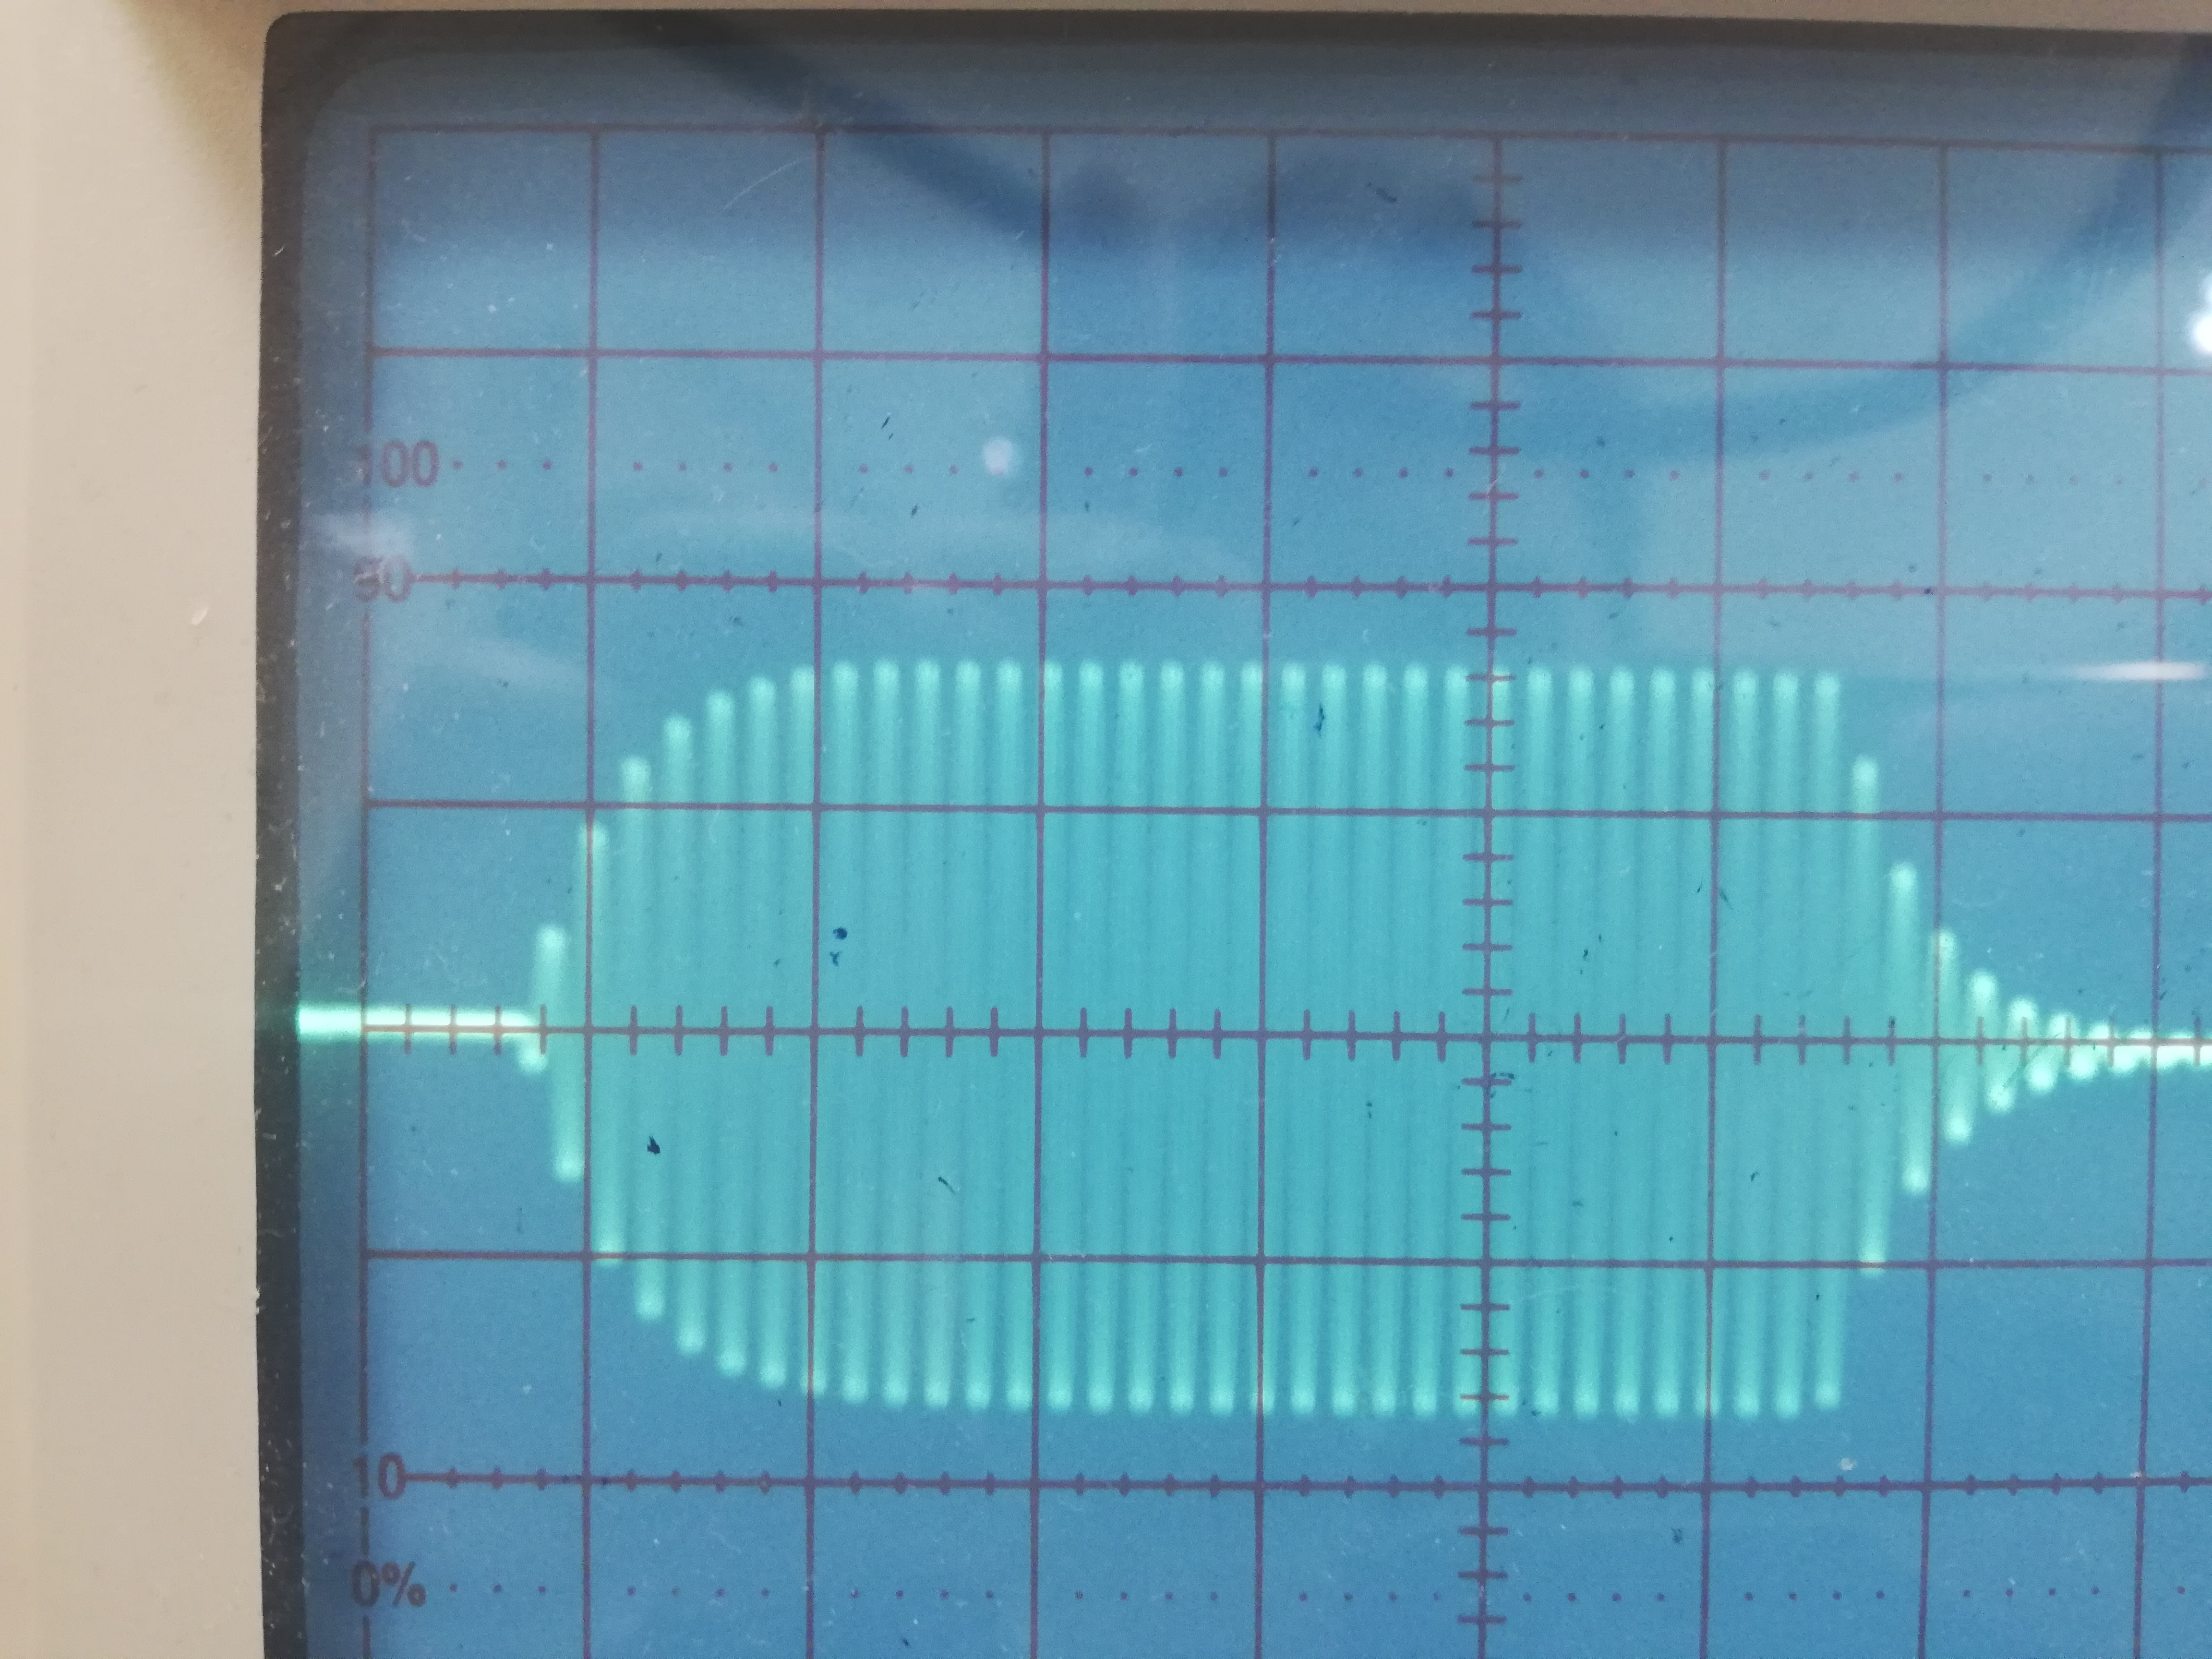
\includegraphics[width=1\textwidth]{2.jpg}

\newpage

\begin{center}
	\large{\textbf{Вывод}}
\end{center}

В работе эксперементально был измерен коэффициент поверхностного натяжения воды, с учетом известного коэффициента поверхностого натяжения спирта. Полученное значение совпадает с табличным по порядку величины, но не совпадает в пределах погрешности. Сильное влияние могло оказать низкая точность поправочного давления на глубине сосуда, неидеальность иглы.

Во чторой части была экспериментально установлена линейная зависимость коэффициента поверхностного натяжения от температуры.



 













 




\end{document}